\chapter{Prototyping}
At the time of writing no research has been done on using motion game controllers as peripherals in a smartphone based biofeedback system. In order to answer the research questions posed in this report it will be necessary to create a simple but working prototype of the aforementioned system. The equipment used to realize the system will be a rooted HTC Desire HD \cite{desireHdSpecs} running CyanogenMod 7 \cite{cyanogenmod} and Wii Remotes with the Motion Plus extension. The application will be created using the Android SDK, Java and the Motej library.

The first section contains documentation of the reverse engineering of the Wii Remote. The second section contains an explanation of the libraries that were used and created for connection. After this the orientation calculation using the Madgwick algorithm is explained in more detail. The fourth section contains documentation and description of the software architectural choices. Next, we demonstrate the final version of the prototype with pictures of the current GUI. Lastly, we discuss the limitations of the application.

\section{Wii Remote Reverse Engineering}
This section will look closer at the reverse engineering of the Wii Remote. Since the Wii Remote is the only sensor to be used in this project, it is important to explain in detail how the data from this sensor is parsed and calibrated. In this section there will be multiple references to Motea. Motea is a lightweight Wii Remote API based on Motej \cite{Motej}, designed specially for this project. A further description of Motea can be found in section~\ref{sec:motea}

Nintendo has not released any documentation on how to connect to, or parse data from the Wii Remote. All the information in this section is taken from internet communities \cite{wiiBrew} that have reverse engineered the Wii Remote and from open source Wii Remote API projects \cite{wiiMoteLib, Motej}.

The Wii Remote is based on the HID protocol for communication, and will appear as such to any host. It is possible to connect to the Wii Remote both with and without Bluetooth pairing. If paired the Wii Remote will attempt to reconnect to the host if the connection is lost. In the current version Motea no pairing is performed. A HID connection is established using L2CAP, by opening a data channel on port 0x13. This channel is used for both sending and receiving data.

\subsection{HID Interface}
The different report types used in the Motea library are displayed in table~\ref{tab:hidInterface}. An output report represents a report that is sent from the host to the Wii Remote. An input report is a report that is sent from the Wii Remote to the host. Input reports are prefixed with 0xA1 and output reports are prefixed with 0xA2. There are more input reports than those listed in table~\ref{tab:hidInterface}, but they are not used by Motea since data report 0x35 contains all the data needed. 

\begin{table}[h!]
\centering
\begin{tabularx}{\textwidth}{|l|l|X|}
\hline
I/O & ID & Description \\ \hline
O & 0x11 & Set LEDs \\ \hline
O & 0x12 & Set data reporting mode \\ \hline
O & 0x15 & Request status information \\ \hline
O & 0x16 & Write to memory/registers \\ \hline
O & 0x17 & Read from memory/registers \\ \hline
I & 0x20 & Status information \\ \hline
I & 0x21 & Data from memory/register request \\ \hline
I & 0x35 & Data report containing data from core buttons, accelerometer and extension (gyroscope) \\ \hline
\end{tabularx}
\caption{\footnotesize The table describes the different output and input reports used by the application}
\label{tab:hidInterface}
\end{table}

A more detailed description on how the output reports work can be found in appendix~\ref{app:outputReports}.

\subsection{Accelerometer}
Accelerometer data is received with every data report of ID 0x35:
\begin{quote}
0xA1 0x35 0xbb 0xbb 0xxx 0xyy 0xzz 0xee 0xee ...
\end{quote}
The data report contains 10 bits of x-axis data, 9 bits of y-axis data, and 9 bits of z-axis data. y- and z-axis data should also be represented as 10 bits, this is done by always letting the least significant bit be 0 for these axes (0bxx xxxx xxx0 where x is some data). The most significant bits of x-, y- and z-axis accelerometer data are located in 0xxx, 0xyy and 0xzz respectively. The least significant bits are located in the 0xbb bytes as shown in figure~\ref{fig:accelerometerData}, these bytes also contain core button data.
\begin{figure}[h!]
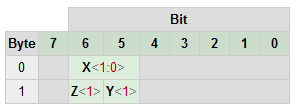
\includegraphics{accelerometerData.png}
\caption{\footnotesize Least significant bits of accelerometer data}
\label{fig:accelerometerData}
\end{figure}

To get the correct G values from the raw accelerometer data, they have to be calibrated. The calibration data is stored in the Wii Remote and can be acquired by sending a read request:
\begin{quote}
0xA2 0x17 0x00 0x00 0x00 0x20 0x00 0x0a
\end{quote}

The Motej \cite{Motej} library did not contain any code for calibrating the accelerometer data. In Motea the calibration is based on an implementation found in the WiiMoteLib \cite{wiiMoteLib} library. Motea parsing and calibrating accelerometer data:
\begin{lstlisting}
// Get raw data
float x = 
	((bytes[4] & 0xff) << 2) | ((bytes[2] & 0xff) >> 5 & 0x03);
float y = 
	((bytes[5] & 0xff) << 2) | ((bytes[3] & 0xff) >> 5 & 0x02);
float z = 
	((bytes[6] & 0xff) << 2) | ((bytes[3] & 0xff) >> 5 & 0x02);

CalibrationDataReport c = source.getCalibrationDataReport();
if (c == null) {
	return;
}

// Calculate calibrated accelerometer data
x = (float) ((x - c.getZeroX()) / 
	(c.getGravityX() - c.getZeroX()));
y = (float) ((y - c.getZeroY()) / 
	(c.getGravityY() - c.getZeroY()));
z = (float) ((z - c.getZeroZ())	/ 
	(c.getGravityZ() - c.getZeroZ()));

source.fireAccelerometerEvent(x, y, z);
\end{lstlisting}

\subsection{MotionPlus}
The MotionPlus extension provides gyroscope data. A complete description on how to connect to, initialize and parse extension data can be found in appendix~\ref{app:gyroParse}.

The gyroscope has two modes: fast and slow. These values tells us what type of scaling to use to get the correct degrees per second. According to WiiBrew \cite{wiiBrew} 20 units from the raw values correspond to 1.45 deg/s in slow mode and 6.59 deg/s in fast mode (e.g. data received with the fast flag on would be multiplied with 1.45/20 = 0.0725 to get the correct degrees per second). Motea uses slightly different values, taken from WiiMoteLib \cite{wiiMoteLib}: 20 units corresponding to 1 deg/s in slow mode and 5 deg/s in fast mode. Which of these values give more accurate data has not been tested, and since the Madgwick algorithm \cite{madgwick} compensates for roll and pitch error using the accelerometer, a small error in the gyroscope data can be tolerated.

\section{Wii Remote library}
In this section we describe Motej and how it was modified to support MotionPlus and connection through Android. We aslo present the new lightweight library, Motea, implemented to replace Motej.

\subsection{Motej and Motejx}
The most complete Java based Wii Remote library that we found was Motej. Work on the library was discontinued in 2009, but supports all the main Wii Remote functionality, and most of its extensions. It was therefore decided to use Motej as the base for a Wii Remote library for Android. 

Using the library is trivial, first you would create an instance of the Mote object, which takes care of handling the connection to the Wii Remote. The Mote constructor takes a string with the Bluetooth address of the Wii Remote to connect to as input. It is also possible to use the MoteFinder class to discover any Wii Remotes that are broadcasting for a connection. The Motej instance fires events whenever it receives data from the Wii Remote, these events can be listened to by implementing the different listeners in the motej.events package. 

Wii Remote extensions are handled by the Motejx library, which is an extension to the Motej library. All supported extensions have to be added to a extensions.properties file, which contains the extension id and the corresponding class that handles the extension. This way Motej does not need to know about the different extension implementations in the Motejx library, because they all implement the Extension interface. To get data from the Wii Remote extensions, a listener has to be added to the extension class.

\subsection{Motej on Android}
\label{sec:motejOnAndroid}
For Motej to work on Android, the BlueCove library has to be replaced with the Android Bluetooth API. This presented a major problem: Wii Remotes use the low level Bluetooth protocol L2CAP to connect to different platforms. As of Android version 4.1, Jelly Bean, \cite{jellyBean} there is no official support for L2CAP. Android only has full support for the higher level protocol RFCOMM.

Though L2CAP is not directly supported through the Android Bluetooth API it is possible to create an L2CAP socket using a technique called reflection:
\begin{lstlisting}
Class<BluetoothSocket> cls = BluetoothSocket.class;
Constructor<BluetoothSocket> constructor = cls.getDeclaredConstructor(
		int.class, int.class, boolean.class, boolean.class,
		BluetoothDevice.class, int.class, ParcelUuid.class);

int type = 3, fd = -1, port = 0x13;
boolean auth = false, encrypt = false;
// Get some device
BluetoothDevice device = getBluetoothDevice();
ParcelUuid uuid = null;

/* type    - Type of socket (3 for L2CAP)
 * fd      - File descriptor (-1 for new socket)
 * auth    - Require authenticaton
 * encrypt - Require encrypted connection
 * port    - Remote port
 * uuid	   - SDP UUID
 */
// This will crate an L2CAP socket on port 0x13
BluetoothSocket socket = constructor.newInstance(type, fd, auth,
		encrypt, device, port, uuid);
\end{lstlisting}

This method has limitations. Because there is no official support for L2CAP in Android, many vendors stock firmware will throw errors when trying to access L2CAP this way. Major vendors such as HTC and Samsung do, as of now, not support L2CAP connections.

\subsection{MotionPlus Support}
Motej supports most of the Wii Remote extensions. Unfortunately, MotionPlus is not one of the supported extensions. MotionPlus was implemented using the already existing extension structure of the Motej library.

Information on how to parse the incoming bytes from the Wii Remote was found on the WiiBrew wiki \cite{wiiBrew}. See appendix~\ref{app:gyroParse} for a more detailed description of how the data is parsed. 

An additional class was added for manual calibration of the gyroscope. There is calibration data stored in the Wii Remote memory, but WiiBrew states that how to use this data for calibration is still unknown. Some suggestions on how to use the data exist, however the calibrated values are not very accurate compared to the manual calibration method. During manual calibration it is required that the Wii Remote is kept still. The calibration takes less than 1 second.

\subsection{Motea}
\label{sec:motea}
During the modification of the Motej library it soon became apparent that several parts of the library were outdated or not optimal for the current application. One problem was discovered when implementing rumbling response to alarm events. The rumble pack was turned off each time a request for status information was sent to the Wii Remote. This bug was caused by the fact that Motej did not modify the status information request with the current status of the rumble pack.

Another issue with the Motej library is that it uses an outdated port to send requests to the Wii Remote. Motej uses the a different channel than 0x13 to send requests. This method only works for the original Wii Remotes, and will not work for the newer models. During testing the original Wii Remote with external MotionPlus was used and therefore this problem was not discovered until later in the development phase.

Because of all the bugs and large portions of the library not being used, we decided to create a lightweight Wii Remote library from scratch and named it Motea. The new library was based on the general structure of our modified Motej library for Android. Much of the code for connecting and parsing data from the Wii Remote was reused. Motea uses the same data pipe, 0x13, for both sending and receiving data from the Wii Remote. Implementing support for the newer type of Wii Remotes should thus prove much simpler.

Currently these input report modes are supported:
\begin{description}
	\item[0x20] Status information
	\item[0x21] Read memory and registers
	\item[0x35] Core buttons, accelerometer, extension data (gyroscope)
\end{description}

Supported output reports are:
\begin{description}
	\item[0x11] Set LEDs and activate rumble pack
	\item[0x12] Set data report mode (only 0x35 will be used)
	\item[0x15] Status information request
	\item[0x16] Write to memory and registers (used for activating MotionPlus)
	\item[0x17] Read memory and registers (for calibration reports)
\end{description}

The new library supports continuous rumbling and connecting the MotionPlus extension while rumbling, which was problematic with Motej. Motea sends requests for status information and checks if a MotionPlus extension is plugged in (if not connected) each second. This allows any class listening to status information events to get regular updates.

\section{Orientation}
In this section we will describe how the orientation of the Wii Remote is calculated using its sensory data.

Two types of data is received: accelerometer data from the Wii Remote and gyroscope data from the MotionPlus extension. The accelerometer data represents the acceleration in each axis, while the gyroscope data represents the rotation around each axis.

There are several algorithms that can be used to calculate the orientation of the Wii Remote. Based on general popularity, and a paper by Tryggestad \cite{Tryggestad} which uses Wii Remote sensor data, we decided to use the Madgwick altitude and heading reference system algorithm (AHRS) \cite{madgwick}. The Madgwick AHRS algorithm uses accelerometer and gyroscope data provided by the sensors to calculate and update the orientation, represented as a quaternion. Magnetometer data can also be utilized to increase the accuracy of the orientation around the z-axis.

Our implementation of the Madgwick AHRS algorithm can be found in appendix~\ref{app:madgwickImplementation}. The implementation was based on a C\# implementation that is available on the x-io Techonologies Limited website \cite{opensourceMadgwick}. 

Quaternions extends the complex numbers, and is therefore hard to explain without using advanced mathematics, which is beyond the scope of this paper. Instead we will focus on describing the input and output of the Madgwick algorithm without going into the calculations. Figure~\ref{fig:orientationProcess} shows how we use the algorithm to calculate the orientation of the Wii Remote. 

The two arrows on the top of the box represents two initial values that need be provided before using the algorithm. \emph{Sample period} is the time between input values. The Wii Remote sends 100 data reports each second and the sample period is therefore 1/100. \emph{Filter gain beta} is used to predict the error rate of the gyroscope data in order to minimize it. The filter gain beta is a constant between 0 and 0.5. In our application we have set this value to 0.5, since the gyroscope data is not very accurate.

The arrows to the left describe the three types of sensor data that can be used to calculate the updated orientation. In our project, magnetometer data is not used because the Wii Remote does not contain this sensor. The box represents the calculations that are done using the input values (accelerometer and gyroscope data in our case). The arrow to the right represents the output of the algorithm. The output is in the form of a quaternion representing the orientation.

\begin{figure}[h!]
  \centering
    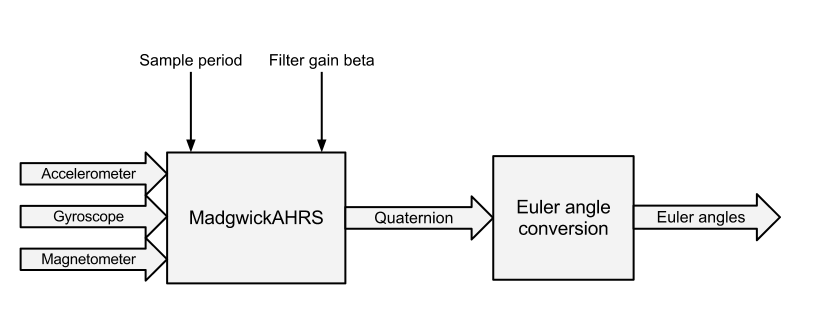
\includegraphics[width=1\textwidth]{orientationProcess.png}
    \caption{\footnotesize The image shows what the input and output variables are for methods used in calcualting the Wii Remote orientation.}
    \label{fig:orientationProcess}
\end{figure}

Since quaternions are hard to understand, we convert the output from the Madgwick algorithm into Euler angles. After the conversion we get three values: pitch, roll and yaw. Pitch, roll and yaw defines the rotation around the x-, y- and z-axis respectively (see figure~\ref{fig:wiiAxis}). It should be noted that the conversion formulas in Madgwick’s paper \cite{madgwick} are incorrect. For the correct conversion formulas see appendix~\ref{app:eulerConversion}

\begin{figure}[h!]
  \centering
    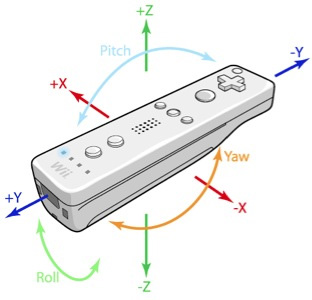
\includegraphics[width=.45\textwidth]{wiimoteAxis.png}
    \caption{\footnotesize A visual representation of the coordinate system for the Wii Remote, taken from the thesis by Tryggestad.\cite{Tryggestad}.}
    \label{fig:wiiAxis}
\end{figure}

\section{Software Architecture}
This section contains an explanation of the various software architectural choices that were made during the implementation of the prototype application. The architecture will be presented from different views, using standard UML diagrams and textual description.

The two main focuses when creating the architecture was \emph{modifiability} and \emph{usability}. By focusing on creating a highly modifiable architecture different parts of the system can be changed without major changes in the overall source code. Creating a modifiable architecture is all about acknowledging that the application may change in the future, and  making the implementation of those changes as painless as possible. This is useful, for example, if we in the future want to add support for multiple Wii Remote input, or use other sensors instead of or in combination with the Wii Remote.

Usability is the other main focus when creating this application’s architecture. Though the current version of the application will not contain a complex graphical user interface (GUI), having usability in mind during the design is important if the code is to be reused in future work. Ultimately a GUI will have to be created for the application to function as intended, and it is therefore important to facilitate for its creation.

\subsection{Architectural Patterns}
\subsubsection{Event-driven architecture}
Event-driven architecture is an architectural pattern that focuses on the creation and consumption of events. The event emitters create new events and push them to the event consumers. The event consumers use the events to produce some reaction. Because event emitters do not directly speak with the event consumers this pattern makes the different components very loosely coupled.

Previously we discussed the importance of modifiability in the software architecture. Using event-driven architecture we achieve high modifiability because of loose coupling between the different components. The event consumers are not concerned with the implementation of the event emitters, therefore as long as the events are on the same form, the only thing that has to be changed is which emitter to listen to. 

The application has been divided into four layers of event emitters. The lowest level sends accelerometer and gyroscope events. In our case these events are created by the Motea library, which handles the connection to the Wii Remote. 

The second level emitter is a handler class for the Wii Remote. This class can easily be edited to handle multiple Wii Remotes if this becomes necessary at a later date. Accelerometer and gyroscope events are consumed and used to create sensor events. These events are designed to stay the same, even if the Wii Remote is replaced by a different sensor.

Sensor events are consumed by a class that uses the sensor data to calculate and update the orientation of the Wii Remote. The updated orientation is then distributed by the third level emitter using orientation events. These events are used to update the 3D-cube in the GUI. 

Orientation events are also consumed by the fourth level emitter, which uses the orientation events to calculate if the angle is steep enough to activate the alarm. The alarm is activated using alarm events.

\subsubsection{Model View Controller}
In the Model-View-Controller (MVC) pattern the code is separated into three main components (see figure~\ref{fig:mvc}): model, view and controller. The view contains the graphical user interface and its logic. The controller updates the model. The model holds the information or state of the application, which is displayed to the user through the GUI. This setup gives the user a mental model that they are interacting with the model directly, even though the model and view are separated in the code.

\begin{figure}[h!]
  \centering
    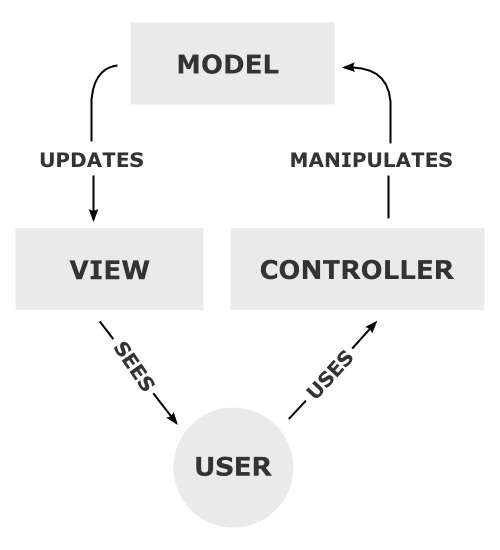
\includegraphics[width=.40\textwidth]{mvc.png}
    \caption{\footnotesize Model View Controller pattern}
    \label{fig:mvc}
\end{figure}

MVC does not directly contribute to the overall usability of the system, but rather seeks to separate the model and the view, improving the modifiability of the GUI. Having the ability to change the GUI continuously throughout the development is paramount for achieve high usability. Using the MVC pattern we can easily change the look and feel of the GUI without interfering with how the model is updated. In our case the model will be changed continuously to reflect the orientation of the Wii Remote.

Because the application is being developed for the Android platform, a strict MVC pattern was not created. User input logic is currently handled by an Android activity. This activity handles button input and Bluetooth discovery of the Wii Remote. It also instantiates other classes when a Wii Remote is discovered. Due to the way Android is constructed, a very strict MVC pattern is not feasible. However, there is still a clear separation between the views, controllers and models using events as described above.

\subsection{Package structure}
Using the discussed patterns as a basis, the following package structure was created, see also figure~\ref{fig:packageDiagram}.

\begin{description}
	\item[libs] Contains the library classes used by the project. Currently only contains the java.swing.event.EventListenerList, which is used by Motea. This class is not included in the standard android packages because swing is not part of android.
	\item[utils] The Motea library, for connecting to the Wii Remote, and our implementation of the MadgwickAHRS algorithm resides here. Motea generates sensor events, while the MadgwickAHRS algorithm is used to calculate orientation.
	\item[models] Classes holding the orientation of the Wii Remote and alarm state of the application are placed here.
	\item[activities] Holds the Android activity classes. The MainActivity class starts the application and handles Android activity events. The CubeView class is used to generate a 3D-model illustrating the orientation of the connected Wii Remote.
	\item[controller] Contains controller classes for interacting with the models and the Wii Remote.
\end{description}

\begin{figure}[h!]
  \centering
    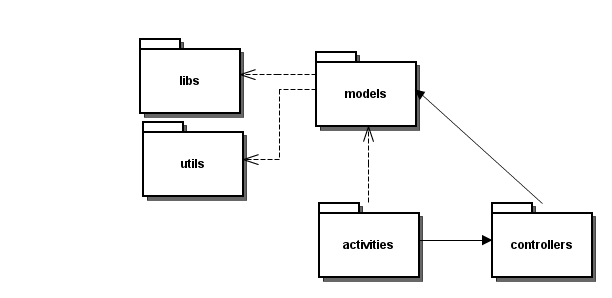
\includegraphics[width=.80\textwidth]{packageDiagram.png}
    \caption{\footnotesize Package diagram}
    \label{fig:packageDiagram}
\end{figure}

\subsection{Activity diagram}
The current application was created to be a proof of concept for the use of Wii Remotes in a mobile biofeedback system. Figure~\ref{fig:activityDiagram} displays the basic functionality implemented in the solution. In addition to the 3D model that graphically displays the orientation of the Wii Remote, an alarm system was implemented. This alarm system is activated when the Wii Remotes angle is greater than some predefined threshold. This threshold  is, as of now, not customizable from the application itself, but is hard-coded  into the application.

The alarm uses sound and vibration to notify the user that the Wii Remote angle has exceeded the threshold. Both sound and vibration is given in pulses with a delay between them, as the Wii Remote angle becomes greater the delay between each pulse decreases. For the vibrotactile feedback the Wii Remote's rumblepack is used and the sound is generated by the Android smartphone speaker. 

\begin{figure}[h!]
  \centering
    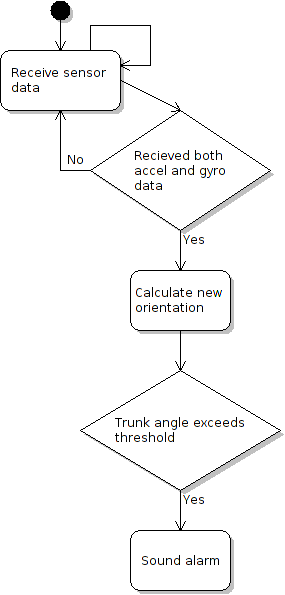
\includegraphics[width=.40\textwidth]{activityDiagram.png}
    \caption{\footnotesize Activity diagram}
    \label{fig:activityDiagram}
\end{figure}

\subsection{Class diagram}
Figure~\ref{fig:classDiagram} shows a class diagram of the application's most important classes. The different background colors represents different parts of the system.

\begin{figure}[h!]
	\centering
	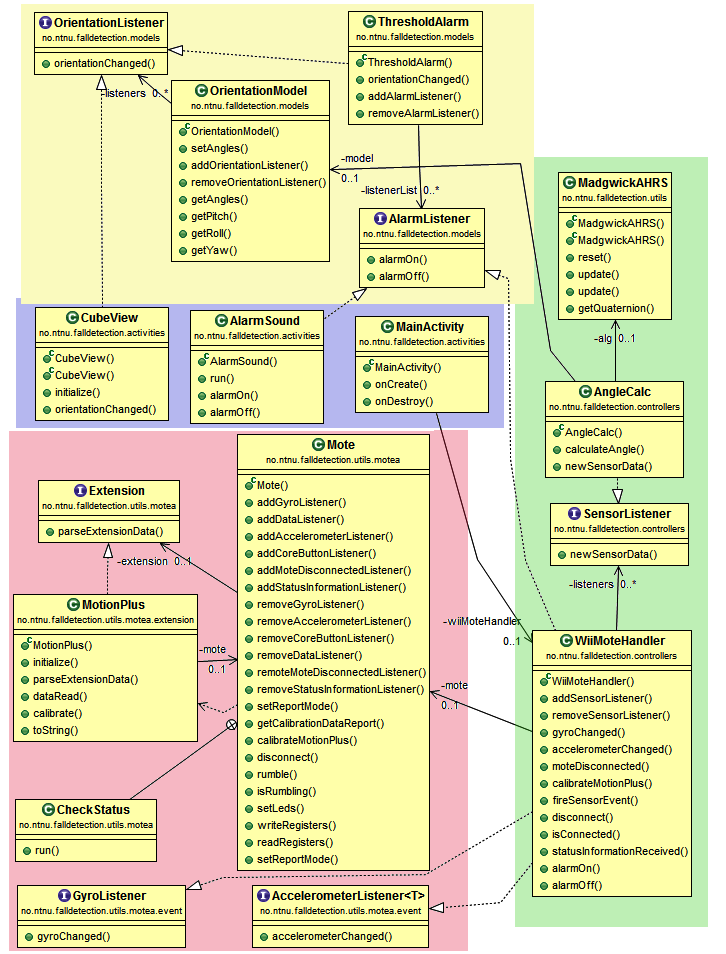
\includegraphics[width=1\textwidth]{classDiagram.png}
	\caption{\footnotesize Class diagram}
	\label{fig:classDiagram}
\end{figure}

The classes with the red background handles the connection to the Wii Remote. When the MainActivity class receives a BluetoothDevice object representing a Wii Remote, that object is used to create an instance of Mote. The Mote class connects to the Wii Remote. Each second the CheckStatus is run to get an update about the Wii Remote's battery life and to connect to and initialize the MotionPlus extension, if it has not already been connected. The MotionPlus class parses the extension bytes received from the Wii Remote, and handles the manual calibration of the gyroscope.

The green background contains the controller classes. WiiMoteHandler handles all communication with the Motea classes (red background). It listens to both the accelerometer and gyroscope events from the Mote instance. When both an accelerometer event and a gyroscope event have been received the WiiMoteHandler fires a sensor event. The WiiMoteHandler listens to alarm events oin order to start the rumblepack in the Wii Remote when the alarm goes off.  A very simple noise cancelling system has been implemented here, to reduce the yaw drift when the Wii Remote is kept still.

AngleCalc listens to sensor events from the WiiMoteHandler, the gyroscope and accelerometer data are used to compute the orientation of the Wii Remote. To compute the orientation AngleCalc uses the Madgwick AHRS algorithm, which is implemented in the MadgwickAHRS class. AngleCalc then updates the OrientationModel with the new orientation data.

The yellow zone holds the models. OrientationModel holds the current orientation of the Wii Remote and fires an event when it is changed. ThresholdAlarm listens to orientation events fired by the OrientationModel and calculates whether the angle is great enough to fire an alarm event. Alarm events have a severity variable that indicates how great the angle is. In the current implementation this variable is to increase the frequency of rumble pulses and sound beeps.

The views have a blue background. MainAcitivty is the class that starts the application. It also handles Bluetooth discovery and initiates the appropriate classes when a Wii Remote is detected. CubeView listens to the orientation events from the OrientationModel to create a graphical representation of the position of the Wii Remote. AlarmSound handles playing beeps from the smartphone when the ThresholdAlarm fires alarm events. 

\section{Prototype application}
The GUI consists of 3 components, two buttons and a visual representation of the Wii Remote. A connection with the Wii Remote is attained by pressing the (1) and (2) buttons on the Wii Remote, and afterwards pressing the "Connect" button on the application. The button will change from "Connect" to "Connecting.." in order to inform the user that it is attempting to establish a connection. Once a connection has been established the "Connect" button will be grayed out an changed to "Connected". A connection is confirmed by the 3D box coming to life, and any movement of the Wii Remote is mirrored by the box on screen. A successful connection will also be indicated on the Wii Remote when the LEDs stop flashing. After a successful connection has been established the LEDs represent battery life. Four lit lights indicated that the battery is full, and one indicates that the battery is nearly empty.

Once a successful connection has been established the Wii Remote should be calibrated in order to achieve optimal accuracy. The Wii Remote calibration constants are not accurate. A rotation of up to 30 rad/s is reported when the Wii Remote is in fact standing still. Through manual calibration this error is reduced to approximately 0. Calibration is achieved by placing the Wii Remote in the desired position and then pressing the "Calibrate" button.

\begin{figure}[h!]
        \centering
        \begin{subfigure}[b]{0.8\textwidth}
                \centering
                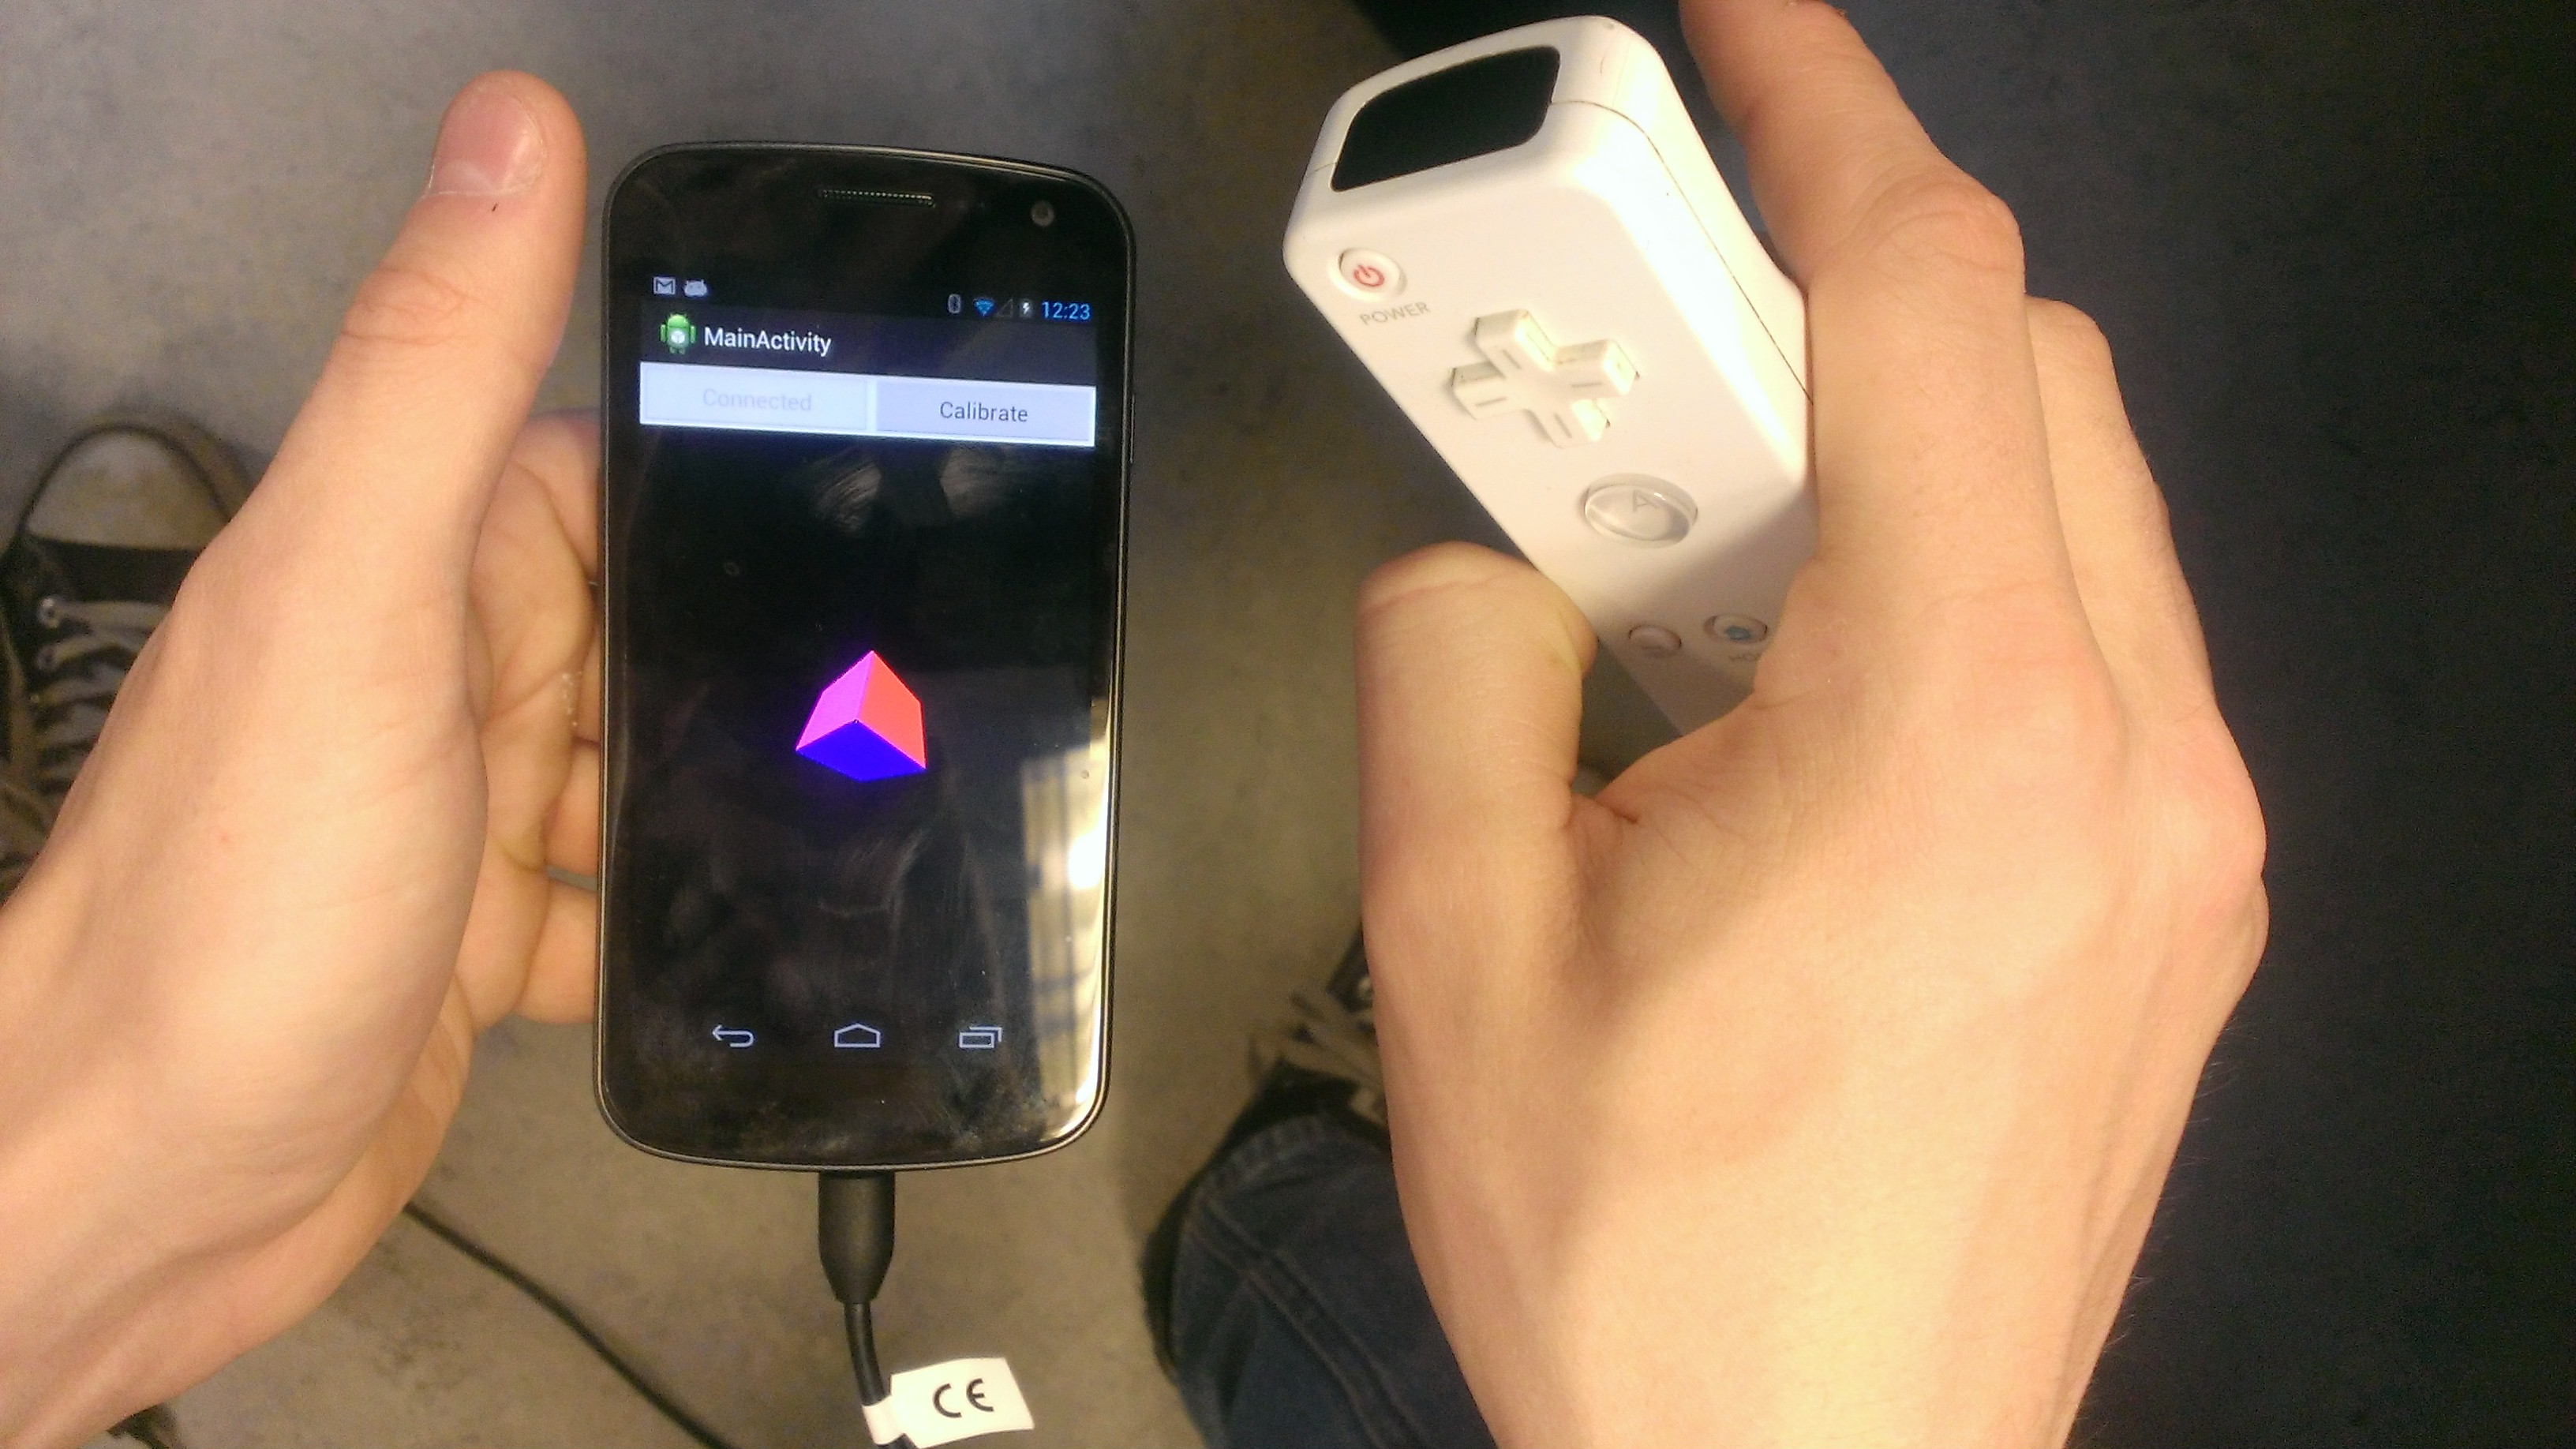
\includegraphics[width=\textwidth]{left.jpg}
                \caption{Wii Remote pointing left}
                \label{fig:left}
        \end{subfigure}
        \\%add desired spacing between images, e. g. ~, \quad, \qquad etc. 
          %(or a blank line to force the subfigure onto a new line)
        \begin{subfigure}[b]{0.8\textwidth}
                \centering
                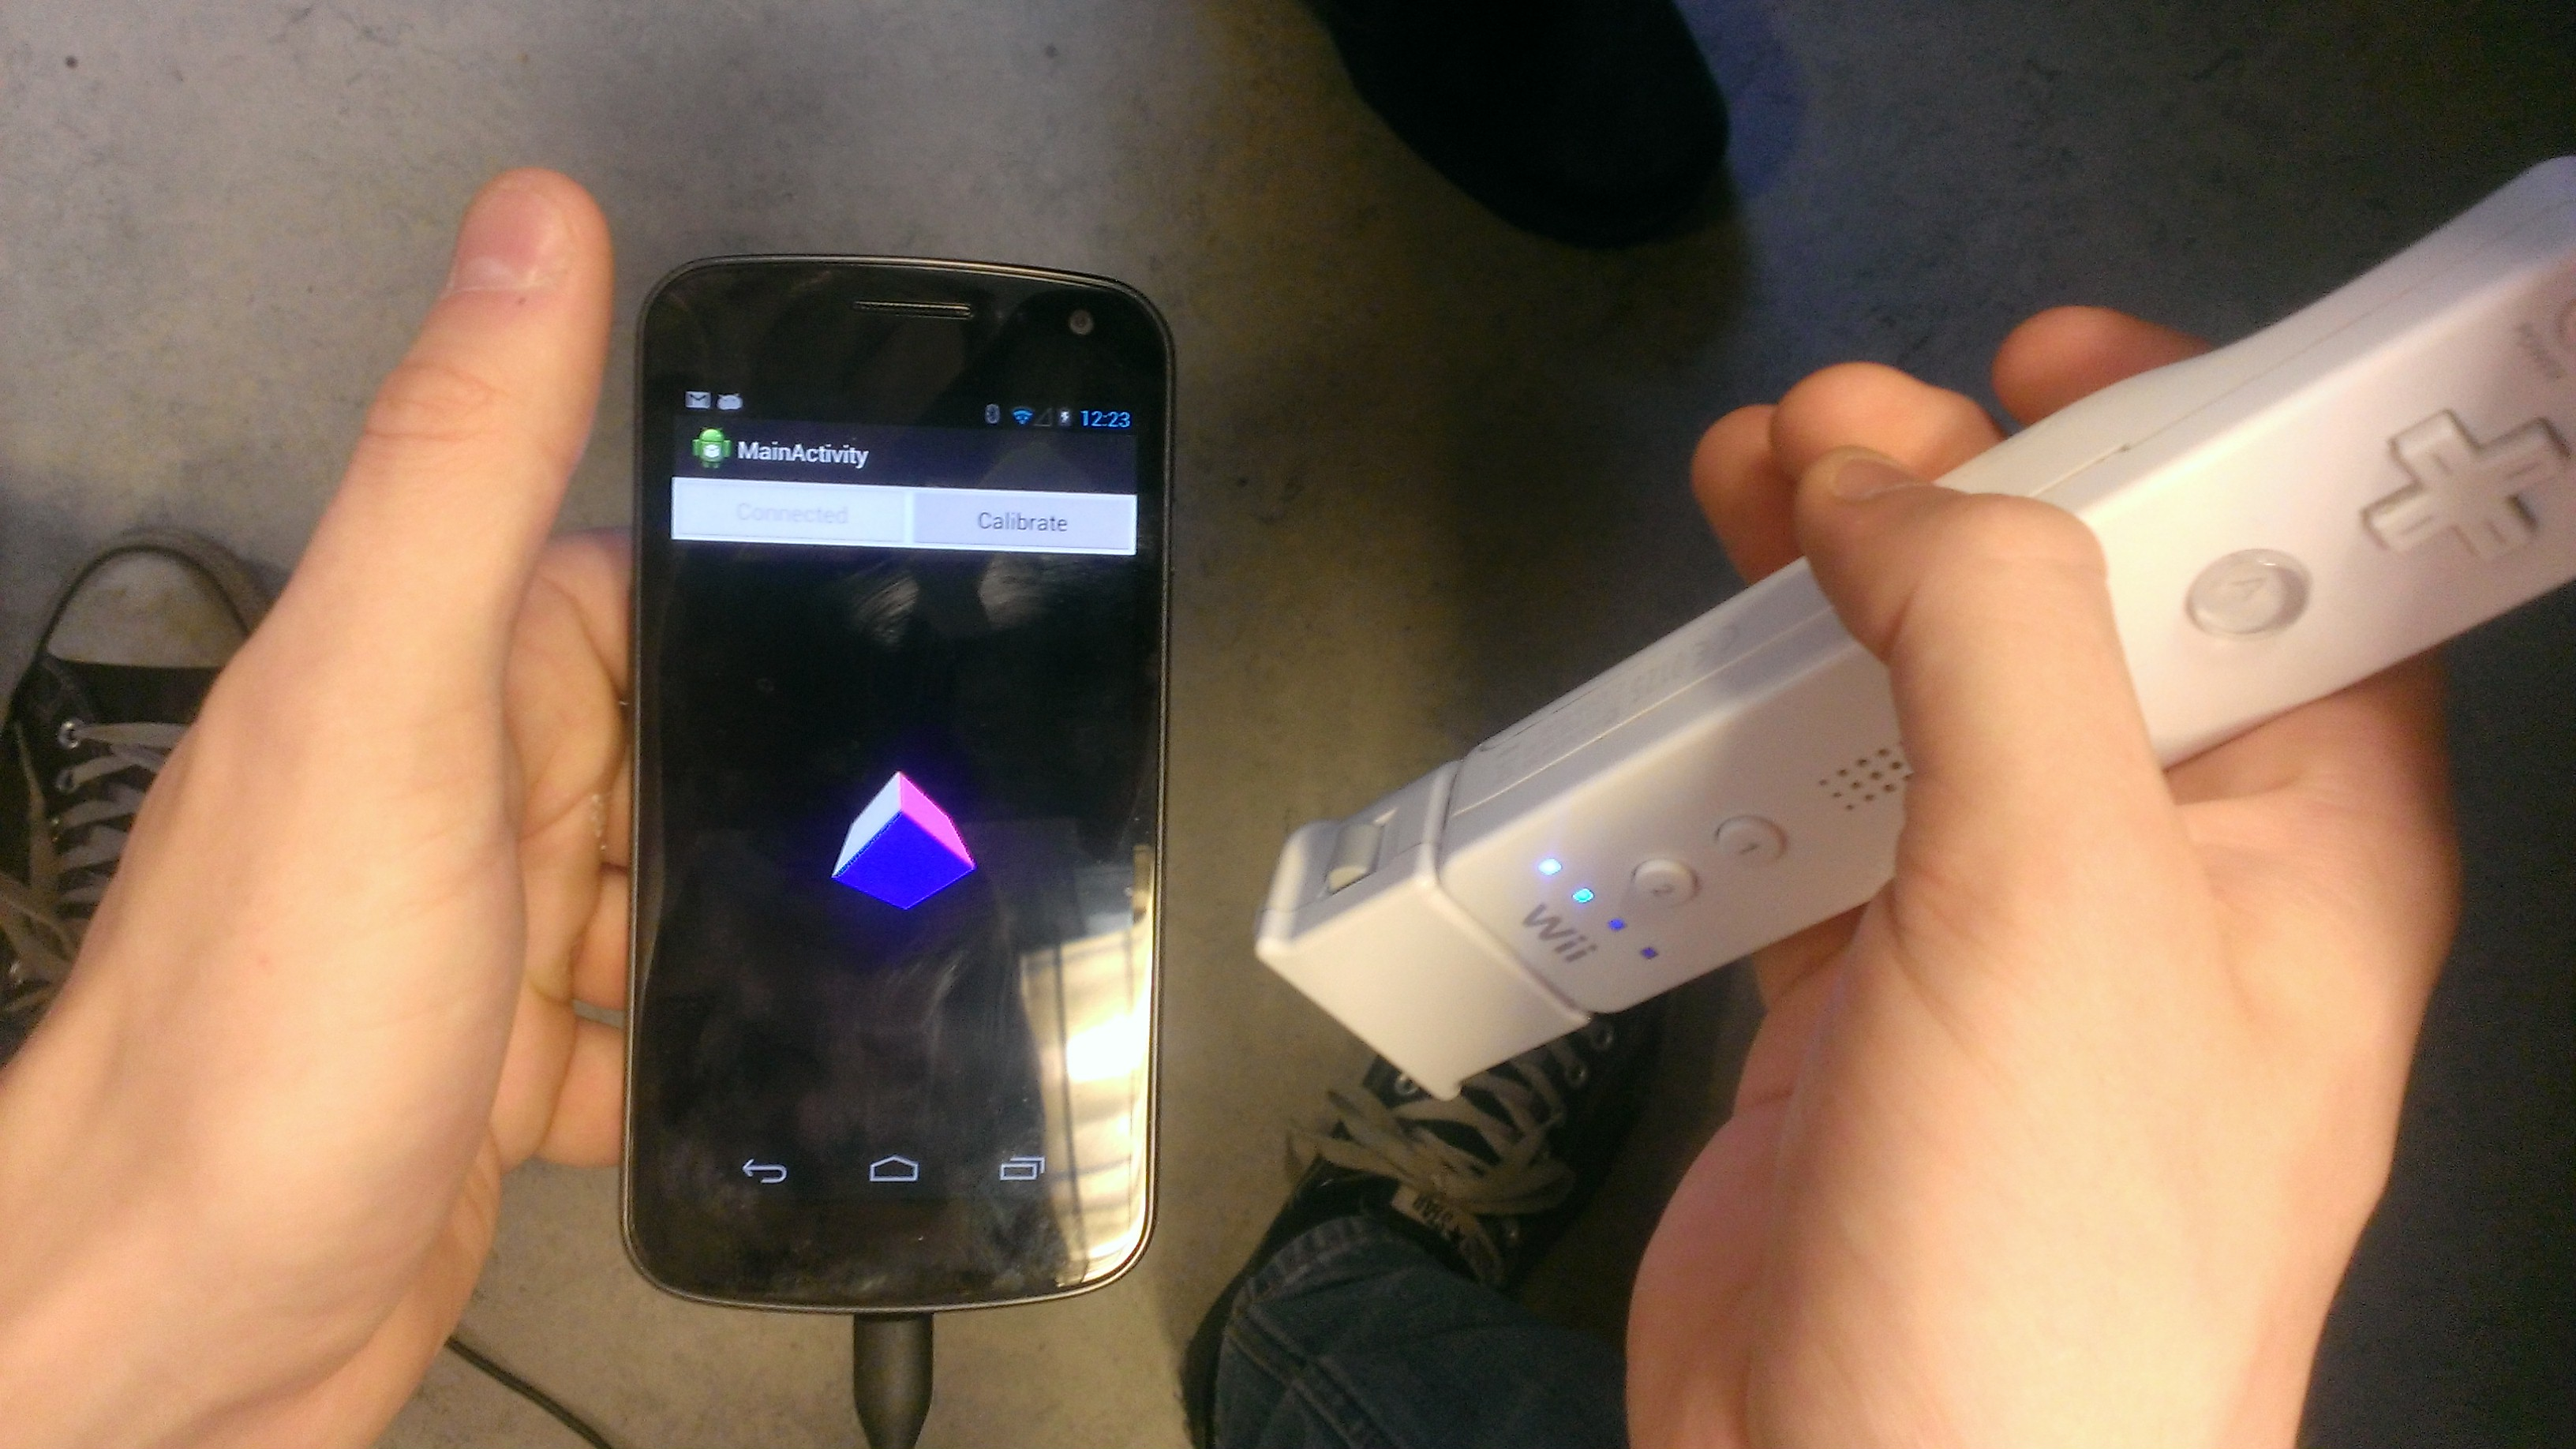
\includegraphics[width=\textwidth]{right.jpg}
                \caption{Wii Remote pointing right}
                \label{fig:right}
        \end{subfigure}
        \caption{Pictures of the application}\label{fig:application}
\end{figure}

The position of the Wii Remote at the time of calibration will be set as the starting point when calculating angular displacement. Once the angular displacement is above the set threshold a beep sound will be activated in set intervals, and the Wii Remote will vibrate in tune with the beeps. The frequency of the vibration and beeps will increase as the angular displacement increases, max intensity is reached at 90 degrees and above.

\section{Limitations}
The current Android SDK does not offer low level support for the Bluetooth stack, including L2CAP. This constraint can be bypassed on some devices by using reflection to access the socket constructor\cite{l2capHtc}. Access could also be gained through using the Android NDK (Native Developer Kit), but we have not tested this approach. Due to L2CAP not being official supported, certain vendors of Android devices have removed the ability to use the L2CAP protocol directly, meaning that it would be impossible to connect to the Wii Remote with stock firmware. The inability to run the prototype on many of todays Android smartphones without replacing the stock firmware is a major limitation of the system.

Another limitation is the lack of testing of availability and performance. Though the informal tests conducted during validity testing suggests that the prototype performs well with respect to availability and performance, additional tests need to be performed in order to confirm that the system will run without errors for longer periods of time.